\documentclass{llncs}
\usepackage{graphicx}

\begin{document}
	
\title{Performance modelling and simulation of skewed demand in complex systems}
\subtitle{Interim Report}

\author{Stephen Shephard SN: 160337206}

\institute{School of Computing Science, Newcastle University, Newcastle upon Tyne, NE1 7RU\\
	\email{s.shephard2@newcastle.ac.uk}}


\maketitle

%
% ---- Introduction
% ---- A short introduction to the project (this should set the scene for the project and motivate why the project is interesting). 
%

\section{Introduction}

There are many high-profile examples of whole IT systems brought down by skewed customer demand for part of their services.  Customers were prevented from using any part of the London 2012 Olympic ticketing website on launch day to avoid demand overloading the system \cite{RN1067}.  HBO Go was brought down by demand for the finale of ``True Detective'' \cite{RN1066}.  Apple's iTunes Store suffered outage on the launch day of the iPhone 7 (new iPhone registration is carried out via an iTunes function) \cite{RN1068}.

It is possible to design and build more resilient systems through effective use of Cloud technologies where higher than normal demand for one function or type of resource would not block access to the others.  Skewed demand may be isolated so that it only affects parts of a system, or shared equally between different components. (The system may also adapt to demand by elastic scaling of resources, but this will be beyond the scope of the project).

In a complex system we need to examine how these components interact.  What impact would a particular choice of middleware have on the demand at the database, for example?  To examine these questions we will choose an approach to build models of selected Cloud technology components that may be combined into different system architectures.

%
% ---- A clear statement of the high-level aim of the project and a list of the scientific objectives of the work. 
%

\section{Aims and Objectives}

We will consider an example system based on the Olympic ticketing use case above.  Such a ticketing application may be generalised to any system for allocating and releasing other resources with variable demand.  Tickets will be for a multi-sport event, and each will consist of a ticket type (the sport), date, row, and seat number.

The system may be implemented using different distributed architectures but all will have the same features.  Users will access the system from a web-based front end.  Tickets will be stored in a database partitioned across several data stores.  In between the web servers and database will be worker applications to service user requests, connected to the web servers by some middleware.

\begin{figure}
	\caption{Ticketing application distributed architecture}
	\centering
	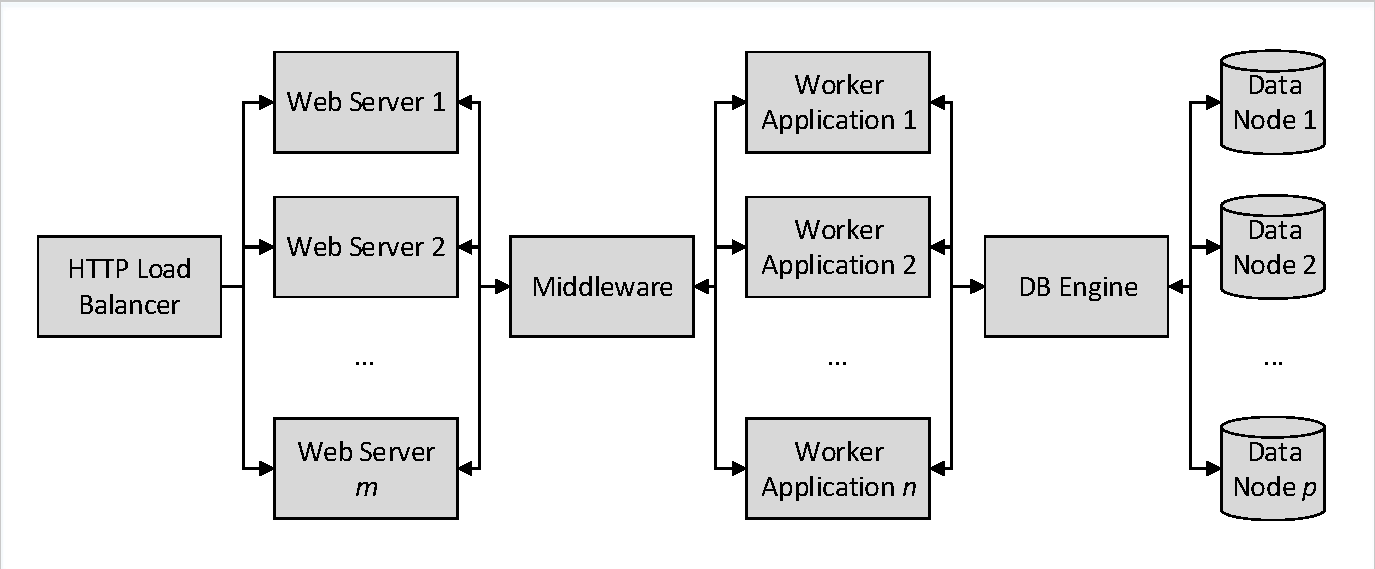
\includegraphics[trim = 5 5 5 5, clip, width=\textwidth]{img/application}
\end{figure}

Models will be built in PEPA (Performance Evaluation Process Algebra) \cite{RN1051} for the following Cloud technology components:

\begin{itemize}
\item Databases
	\begin{itemize}
	\item Separate databases
	\item Distributed database nodes using horizontal partitioning \cite{RN68}
	\item Distributed database nodes with Cassandra-style replication \cite{RN1050}
	\end{itemize}
\item Shared middleware queue \cite{RN65}
\item Event streaming application for eventual consistency architectures \cite{RN1071}
\end{itemize}

The PEPA component models will be tested then composed into a set of different system architectures below, which will also be built on the Microsoft Azure platform.  Both the models and real systems will be tested under different scenarios of skewed demand.

\begin{description}
	\item[Simple microservices] Two separate databases, one for Athletics tickets, one for Cycling.
	\item[Operational microservices] A more `natural' microservices architecture partitioning the system by operation (Book, Search, Return) with a separate database for each.  The databases maintain eventual consistency via an event streaming application e.g. using Kafka.
	\item[Shared queue middleware] Requests via a shared queue to worker applications going to a distributed database with two nodes, Athletics and Cycling.
	\item[Distributed database with replication] Requests via a shared queue to worker applications going to a distributed database with three nodes, Athletics, Cycling and Diving, where each partition is replicated on another node.
\end{description}

\paragraph{Objectives.}  The objectives are to determine whether or not PEPA models of the components examined, once composed into architectural models:
\begin{itemize}
	\item are good predictors of the behaviour of real systems under skewed demand scenarios
	\item provide insights into the effectiveness of Cloud technologies for handling skewed demand.
\end{itemize}

%
% ---- A brief description of the progress so far made (i.e. areas researched, analysis undertaken, software or model development undertaken). 
%

\section{Progress}

\begin{tabular}{ p{0.1\textwidth} p{0.85\textwidth} }
	Done & Task \\
	\hline
	15/03 & Completed ``Investigating Cloud Technologies to Maximise Availability of Oversubscribed Resources'' for Research Skills module \\
	25/04 & Agreed initial scope of ``Performance modelling and simulation of skewed demand in complex systems'' \\
	05/05 & Documented first outline plan in GitHub \\
	08/05 & Submitted Ethics form \\
	31/05 & Produced PEPA models for all except Event Streaming component and Operational Microservices archiecture
\end{tabular}

%
% ---- A timed work plan for completion of the project.
%

\section{Plan}

\begin{tabular}{ p{0.1\textwidth} p{0.1\textwidth} p{0.75\textwidth} }
	Start & Due & Task \\
	\hline
	05/06 & 16/06 & Produce interim report \\
	.. & .. & .. \\
	03/08 & 09/08 & Produce presentation \\
	10/08 & 11/08 & Attend presentation \\
	12/08 & 25/08 & Update and submit final version of dissertation \\
\end{tabular}

%
% ---- Bibliography ----
%

\bibliographystyle{splncs03}
\bibliography{references}

\end{document}